%\section{Commonsense Knowledge Types}
\label{knowledge_types}
Intrigued by the remarkably achieved accuracy of the Sharma and Baral \cite{2018CommonsenseKT} approach, we now describe this work in more details. In the previous chapter, in section \ref{section:TheDifferentApproaches} we outlined \ref{Steps} of the approach. Here, we first focus on the process of identification of the presented commonsense knowledge types. Then, we discuss the proposed reasoning algorithm and the provided worked out example. We conclude this chapter with some final observations about this approach.


\section{Identification of Commonsense Knowledge Types}
The first step of the Sharma and Baral \cite{2018CommonsenseKT} approach is to represent the input Winograd sentence and question as semantic graphs. To achieve this, the KParser from \cite{DBLP:conf/ijcai/SharmaVAB15} is used. 
To illustrate the results of the semantic parsing, we now analyze the graphs for the sentence and question from \ref{ex:Graph} which are shown in Figure \ref{Graph11} and Figure \ref{Graph12}. \\ 
\labeltext{\textit{Example 3.1.1}}{ex:Graph}
\begin{itemize}
	\item[\textbf{S:}] \textbf{The man could not lift his son because he was weak.}
	\item[\textbf{Q:}] \textbf{Who was weak?}
\end{itemize}

In these graphs, the different colors of the nodes indicate the predefined class of nodes to which they belong. 
Nodes with red color represent events which correspond to the verbs in the sentence. Nodes with blue color represent entities and qualities of entities, and the nodes with gray color represent conceptual classes. The labels on the directed edges are the semantic relations between the different nodes in the graph. The number next to a word refers to the position of the word in the sentence. 
\begin{figure}
	\centering
	%\documentclass[border=10pt]{standalone}
%\usepackage{tikz}
\tikzset{
	treenode/.style = {shape=rectangle, rounded corners,
		draw, align=center,
		top color=white, bottom color=blue!20},
	root/.style     = {treenode, font=\ttfamily\normalsize, bottom color=red!30},
	env/.style      = {treenode, font=\ttfamily\normalsize},
	dummy/.style    = {circle,draw},
	level 1/.style={sibling distance=6cm, level distance = 3em, label = 1pt },
	level 2/.style={sibling distance=2.3cm,level distance = 5em}, 
	level 3/.style={sibling distance=2cm},
	blueRed/.style={env, top color=blue, bottom color=red} 
}
%\begin{document}
	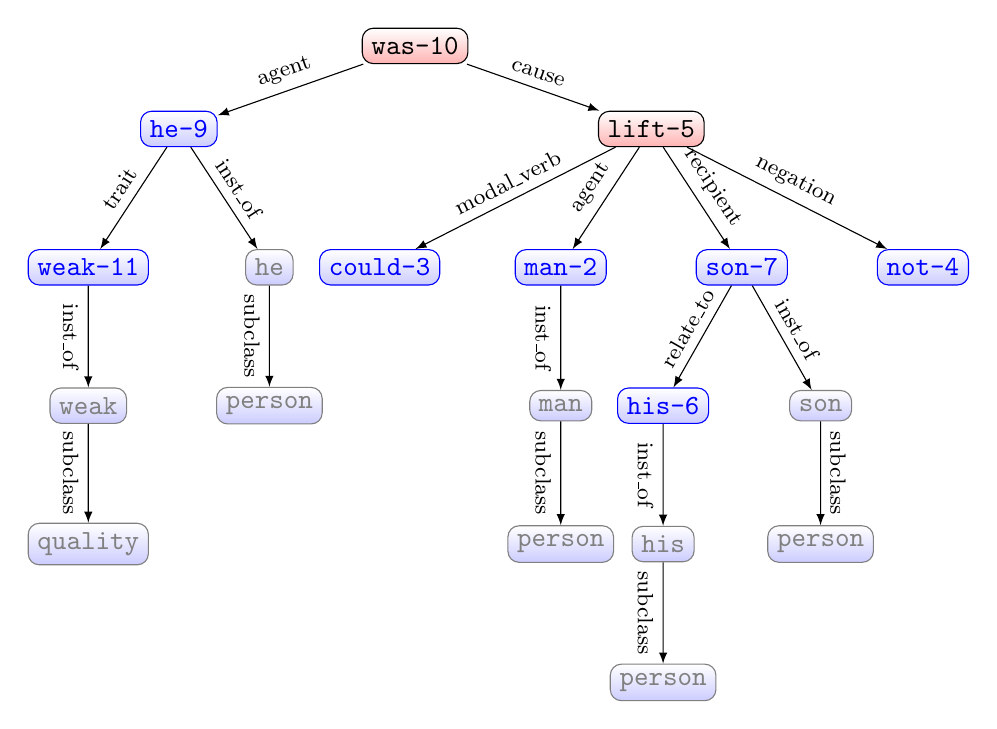
\begin{tikzpicture}
	[
	grow                    = down,
	sibling distance        = 50em,
	level distance          = 5em,
	edge from parent/.style = {draw, -latex},
	every node/.style       = {font=\footnotesize},
	sloped
	]
	\node [root] {was-10}
	child { node [env, blue] {he-9}
	  child {node [env, blue] {weak-11}
	  	 child {node [env, gray] {weak}
	  		child {node [env, gray] {quality}
	  			edge from parent node [below] {subclass}}
	  		edge from parent node [below] {inst\_of}}
			edge from parent node [above] {trait}}
	  child {node [env, gray] {he}
	  		child {node [env, gray] {person}
	  			edge from parent node [below] {subclass}}
	  		edge from parent node [above] {inst\_of}}	
	   edge from parent node [above] {agent}}
	child { node [env, bottom color=red!30] {lift-5} 
	  child {node [env, blue]  {could-3}
	  	edge from parent node [above] {modal\_verb} }	
	  child {node [env, blue]  {man-2}
	  	child {node [env, gray] {man}
	  		 child {node [env, gray] {person}
	  			edge from parent node [below] {subclass}}
	  		edge from parent node [below] {inst\_of}}
	  	edge from parent node [above] {agent} }
	  child {node [env, blue]  {son-7}
	  	child {node [env, blue] {his-6}
	  		child {node [env, gray] {his}
 			  	child {node [env, gray] {person}
  				   edge from parent node [below] {subclass}}
	  			edge from parent node [below] {inst\_of}}
	  		edge from parent node [above] {relate\_to}}
  		child {node [env, gray] {son}
  			child {node [env, gray] {person}
  				edge from parent node [above] {subclass}}
  		 edge from parent node [above] {inst\_of}}
	  	edge from parent node [above] {recipient}}
	  child {node [env, blue]  {not-4}
			edge from parent node [above] {negation} }
		edge from parent node [above] {cause}};
	

	\end{tikzpicture}
%\end{document}
	\caption{\label{Graph11}``The man couldn't lift his son because he was so weak."}
\end{figure}


\begin{figure}
	\centering
	%\documentclass[border=10pt]{standalone}
%\usepackage{tikz}
\tikzset{
	treenode/.style = {shape=rectangle, rounded corners,
		draw, align=center,
		top color=white, bottom color=blue!20},
	root/.style     = {treenode, font=\ttfamily\normalsize, bottom color=red!30},
	env/.style      = {treenode, font=\ttfamily\normalsize},
	dummy/.style    = {circle,draw},
	level 1/.style={sibling distance=3cm, level distance = 3em},
	level 2/.style={sibling distance=1.7cm,level distance = 5em}, 
	level 3/.style={sibling distance=2cm},
	blueRed/.style={env, top color=blue, bottom color=red} 
}
%\begin{document}
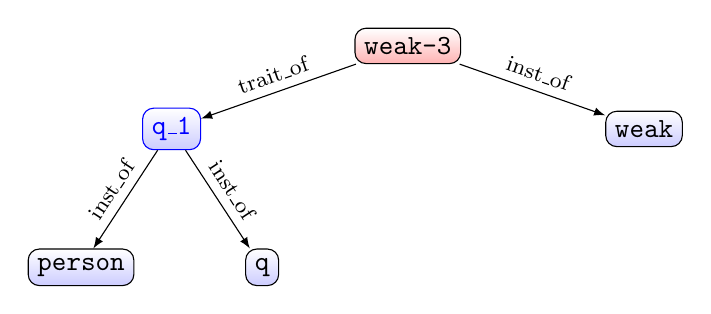
\begin{tikzpicture}
[
grow                    = down,
sibling distance        = 50em,
level distance          = 5em,
edge from parent/.style = {draw, -latex},
every node/.style       = {font=\footnotesize},
sloped
]
\node [root] {weak-3}
child { node [env, blue] {q\_1}
	child {node [env] {person}
		edge from parent node [above] {inst\_of}}
	child {node [env] {q}
		edge from parent node [above] {inst\_of}} 	
	edge from parent node [above] {trait\_of}}
child {node [env] {weak}
		edge from parent node[above] {inst\_of}};


\end{tikzpicture}
%\end{document}
	\caption{\label{Graph12}``Who was weak?"}
\end{figure}

For the representation of the question, one additional conceptual class labeled as "q" is introduced. In this conceptual class are all nodes which represent the question words from the WSC problems, such as: \textit{Who, Which and What}.

From the observation of these two graphs, Sharma and Baral \cite{2018CommonsenseKT} come to conclusion that the missing knowledge required to answer the question, must connect the trait of an entity being weak with its inability to lift. In Figure 3 is the representation of this knowledge as shown in \cite{2018CommonsenseKT}. 

%TODO add here graph for their type
\begin{comment}
	content...

\begin{figure}
	\centering
	%\documentclass{standalone}
%\usepackage{tikz}
%\usetikzlibrary{arrows, shapes, trees, positioning}

%\begin{document}
	
	\tikzset{
		treenode/.style = {shape=rectangle, rounded corners,
			draw, align=center,
			top color=white, bottom color=blue!20},
		root/.style     = {treenode, font=\ttfamily\normalsize},
		env/.style      = {treenode, font=\ttfamily\normalsize},
		dummy/.style    = {circle,draw},
		level 1/.style={sibling distance=6.3cm, level distance = 6em},
		level 2/.style={sibling distance=2.5cm,level distance = 5em}, 
		level 3/.style={sibling distance=2cm},
		blueRed/.style={env, top color=blue, bottom color=red} 
	}
	
	\begin{tikzpicture}
	[
	grow                    = down,
	sibling distance        = 50em,
	level distance          = 5em,
	edge from parent/.style = {draw, -latex},
	every node/.style       = {font=\footnotesize},
	sloped
	]
	
	
	
	% Theraspist 1
	\node[root]   (root)   {weak-1}
	child {node [env, gray] {weak}
		edge from parent node [above] {inst\_of}}
	child {node [env, gray] (s1) {y-2}
		child {node [env, gray] {entity}
			edge from parent node[above] {inst\_of}}
		edge from parent node[above] {is\_trait\_of}
	} ;
	
	
	
	% Theraspist 2
	\node[root]   (lift)   [right=45mm of root] {lifts-5}
	child {node [root] (s1) {y-2}
		edge from parent node[above] {agent}}
	child {node[env, gray] (S4) {lift}
		edge from parent node[above] {inst\_of}};
	
	\draw[-> ] (root) -- node[above] {prevents} (lift);
	%\draw[-> ] (lift) -- node[above] {agent} (s1);
	
	\end{tikzpicture}
%\end{document}
	\caption{\label{Graph13}``Prevents type?"}
\end{figure}
\end{comment}

By applying this observation to all problems from the WSC corpus, Sharma and Baral \cite{2018CommonsenseKT} identified 12 different knowledge types. From these, the first 10 knowledge types share the same structure as they are all based on different interactions between actions and properties. Each of the 10 knowledge types consists of three parts: the first and third part are sentences containing entities, properties or actions, whereas the second part is a semantic relation (\textit{causes, prevents} or \textit{followed by}) which connects them. The last two knowledge types have different structure because one of them requires multiple knowledge and the other one is based on the conditional likelihood of a previous event. 
For the representation of the knowledge type shown in Figure 1.3, the first part is \textit{weak y}, the third part is \textit{y lifts} and the semantic relation is \textit{prevents}.
The presented knowledge types are the following:

\begin{quote} 
	Property \textit{prevents} Action, Action1 \textit{prevents} Action2, Action1 \textit{causes} Action2, Property \textit{causes} Action, Action \textit{causes} Property, Property1 \textit{causes} Property2, Action1 \textit{followed by} Action2, Action \textit{followed by} Property, Property \textit{followed by} Action, Co-existing Action(s) and Property(s), Statement1 \textit{is more likely than} Statement2, Multiple Knowledge. 
\end{quote}


\section{Reasoning Algorithm}
In this section we explain the proposed logical Reasoning Algorithm (RA) from Sharma and Baral \cite{2018CommonsenseKT}. This RA was used for solving the WSC problems by applying the previously explained knowledge types. It takes a formal representation of Winograd sentence and question and additional knowledge as input and it returns an answer to the question. The implementation of the RA together with a running example is available online\footnote{https://drive.google.com/file/d/1WN0T98HaMFhWEEIH-3AlWoIPxAdFYlT\_/view}. The implementation of the RA  can be also found in Appendix\ref{AppendixA}. 

The RA is based on Answer Set Programming (ASP) \cite{DBLP:conf/aaai/Lifschitz08}. Therefore, after the Winograd sentence and question have been represented as semantic graphs, the observations from these graphs are encoded as ASP rules. The retrieved answer should be entailed by these input rules.
The RA is split into two main phases, each including several steps. Each step, results in creating new ASP rules.
\begin{itemize}
	\item \textbf{Phase 1: Generating merged representation}\\
	 In this phase, the graph representation of the Winograd sentence and the additional knowledge are merged. The idea here is to extend the information from the input sentence with the information from the additional knowledge. To achieve this, the following information from both graph representations is extracted and later merged.
	\begin{enumerate}
		\item All the nodes which are an instance of a defined class of nodes (for example: person, motion, description) in the KParser are identified as constant nodes. All constant nodes have a directed edge labeled as \textit{instance\_of} to another node in the graph. 
		\item Constant nodes with parents/children as constant nodes are identified. These are nodes previously identified as constant nodes which have directed edges to other constant nodes.
		\item The cross domain siblings in both representations are identified. These are different constant nodes which appear in both graphs and they both are instances of nodes of the same type. 
		\item Nodes which are identical in both graphs are identified. These nodes are called cross domain clones and are of the same type as the cross domain sibling. Additionally, they have the same number of child/parent nodes which are connected through the same semantic relations. 
		\item In this last step a merged representation is created. The merged representation is a copy of the sentence's representation, expanded with the additional knowledge by adding edges between nodes from both graphs that have been identified as cross domain clones.
	\end{enumerate}

	\item \textbf{Phase 2: Extracting possible answers}\\
	In this phase, the graph representation of the WSs question is projected onto the merged representation from the previous step. The goal is to retrieve the nodes which are cross domain clones of the unknown node (q) from the question in the merged representation. Similarly as in the previous phase, information from both graph representations is extracted and merged.
	\begin{enumerate}
		\item Constant nodes are identified from both graphs.
		\item Nodes with children/parent as constant node are identified. 
		\item Cross domain siblings of the nodes from the question graph are \\ identified in the merged representation.
		\item Using the previously extracted nodes, the cross domain clones of the nodes from\\ the question graph are identified in the merged representation.
		\item Nodes from the merged graph which are cross domain clones to the unknown node (q)\\ from the question graph are retrieved as an answer.
	\end{enumerate}
\end{itemize}

According to Sharma and Baral \cite{2018CommonsenseKT} this RA can be applied to the first 10 from the 12 identified knowledge types.

\paragraph{Worked-out example} To verify the work of the RA, we tried the worked out example which was provided together with the implementation in the supplementary document for Sharma and Baral \cite{2018CommonsenseKT}. The worked out example includes the ASP encoding of the sentence and question from \ref{ex:Graph}. For extraction of additional knowledge the sentence \textit{``She could not lift it because she is a weak girl"} was used. The extracted knowledge is from the first type which was analyzed before \textit{``weak y prevents y lifts"} and this has also been provided in ASP encoding. Running the RA with the provided ASP rules for the sentence, question and knowledge type, retrieves as an answer: \textit{ans(q\_1,he\_9)} and \textit{ans(q\_1,man\_2)}. Hence, the two nodes \textit{he\_9} and \textit{man\_2} from the merged representation correspond to the unknown node \textit{q\_1} from the question. The conclusion is that the correct referent for the ambiguous pronoun \textit{he\_9} in this case is the noun \textit{man\_2}. 

\paragraph{Observations}
After trying the provided worked out example and ensuring that the RA retrieved the correct answer, we decided to test the RA with some more WSC problems. %TODO add here the number of the WS problems we encoded in ASP  
In order to do this, we followed the steps for the worked out example. We first used the KParser to get the graph representation of the input Winograd sentence and question and after that we encoded this representation in ASP format. Since the knowledge types for the different WSC problems are not publicly available, we could not know which problem from which knowledge type is. Therefore, the encoding for the additional knowledge remained the same. Nevertheless, for all the WSs that we encoded the correct answer was retrieved. 
What came as a surprise is that even for the worked out example, after the rule that defines the knowledge type is commented out, again a correct answer is retrieved. Therefore, we can conclude that the RA does not use the rule for the knowledge type in the reasoning process. Rather, it relies on hard coded information about the agent and the recipient of the action for retrieving the answer. 

All things considered, the approach by Sharma and Baral \cite{2018CommonsenseKT} provides different categories of knowledge types but in our opinion, in the reasoning process these knowledge types are not considered at all.  The encoded knowledge type is not sufficient?
%TODO maybe add here one concluding sentence

